% !TeX root = ../main.tex
% Add the above to each chapter to make compiling the PDF easier in some editors.

\chapter{Introduction}\label{chapter:introduction}
In this chapter, the theoretical background of the thesis is written. First, the basics of X-ray radiography is introduced, then Digital Subtraction Angiography (\gls{dsa}) is described briefly and it is shown how Digital Variance Angiography (\gls{dva}) differs from the prior approach. Next, it is shown how intensity transformations can be utilized to enhance crucial image features. Later, spatial and frequency domain filtering techniques are presented. In the end of the chapter, further methods are discussed which do not fall into the previously mentioned categories.

\section{X-ray Radiography}
X-ray radiography is a powerful tool used in medical imaging. It is a non-invasive imaging technique that uses a beam of X-rays to create an images of the inside of the body relatively fast. X-ray is a form of electromagnetic radiation which has a wavelength ranging from about $10^{-8}\:m$ to $ 10^{-12}\:m$ (from $3\:\cdot\:10^{16}\:Hz$ to $3\:\cdot\:10^{19}\:Hz$) and energy between 20 - 120 $keV$ \cite{rontgen1896new}. 

There are several interactions possible when X-rays interact with matter \cite{seibert2005x}. Here we only discuss the effects of photoelectric absorption and Compton scattering to beam attenuation as these are the most dominant factors in the energy range of medical imaging (Figure \ref{fig:cross-section}).

\begin{figure}[htpb]
  \centering
  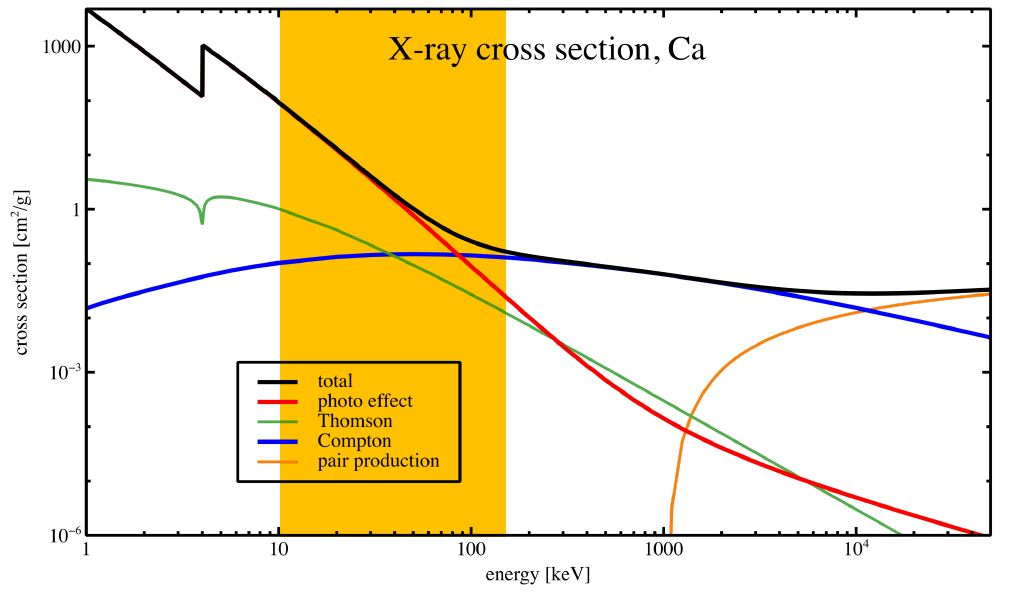
\includegraphics[width=0.8\textwidth]{figures/intro/cross-section.JPG}
  \caption{Various X-ray cross sections as function of energy for Calcium} \label{fig:cross-section}
\end{figure}

Assuming an inhomogeneous sample and a monoenergetic beam, Lambert-Beer's law can be expressed as:
\begin{equation}
    I(d)=I_0\cdot\exp(-\int_{0}^{d}\mu(s)\cdot d(s))
    \label{eq:labmert-beer}
\end{equation}
\begin{equation}
    p(d)=-\ln(\frac{I(d)}{I_0})=\int_{0}^{d}\mu(s)\cdot ds
    \label{eq:line-integral}
\end{equation}


\emph{p(d)} is called the line integral. \emph{I(d)} is the intensity in distance \emph{d} behind the initial intensity \emph{I(0)}. \emph{\textmu (s)} is the mass attenuation coefficient, which is composed by cross sections of different interactions. In X-ray radiography, the beam is leaving the X-ray tube with the initial intensity \emph{I(0)}, then interacts with tissues of various mass attenuation coefficients (\emph{\textmu (s)}).  As it reaches the detector, the initial intensity is reduced to \emph{I(d)}.

Based on equation \ref{eq:line-integral}, it can be explained that materials with higher \emph{\textmu} values are more visible on X-ray images. In the human body, these materials with high \emph{\textmu} are mostly bones. Figure \ref{fig:attenuation-for-bone-and-tissue} compares \emph{\textmu} of bones and soft tissue. In the diagnostic energy range, bone contributes the most significantly to the total attenuation, therefore it is the most visible tissue on the final image.

\begin{figure}[htpb]
  \centering
  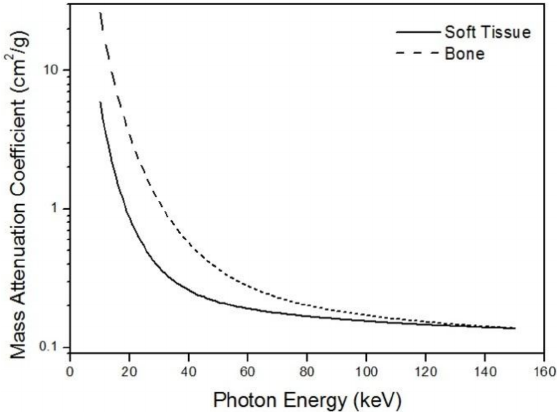
\includegraphics[width=0.5\textwidth]{figures/intro/attenuation-for-bone-and-tissue.png}
  \caption{The mass attenuation coefficient as a function of photon energy for bone and soft tissue within the diagnostic energy ranges (30–150 $keV$) \cite{kim2013optimal}} \label{fig:attenuation-for-bone-and-tissue}
\end{figure}

As a conclusion, visualizing vessel structure is not possible using traditional X-ray radiography. To solve this issue, angiography has been evolved.

\section{Angiography}
In Angiography, a contrast agent is injected into the blood vessel. On of the most popular types of these contrast agents are iodine-based contrast media. As Figure \ref{fig:attenuation-for-several-materials} shows, the mass attenuation coefficient of iodine is relatively high compared to the tissues in the human body. Utilizing this attribute of iodine, visualization of vessels is possible for that short time when the contrast agent expands in the human body right after injection.

\begin{figure}[htpb]
  \centering
  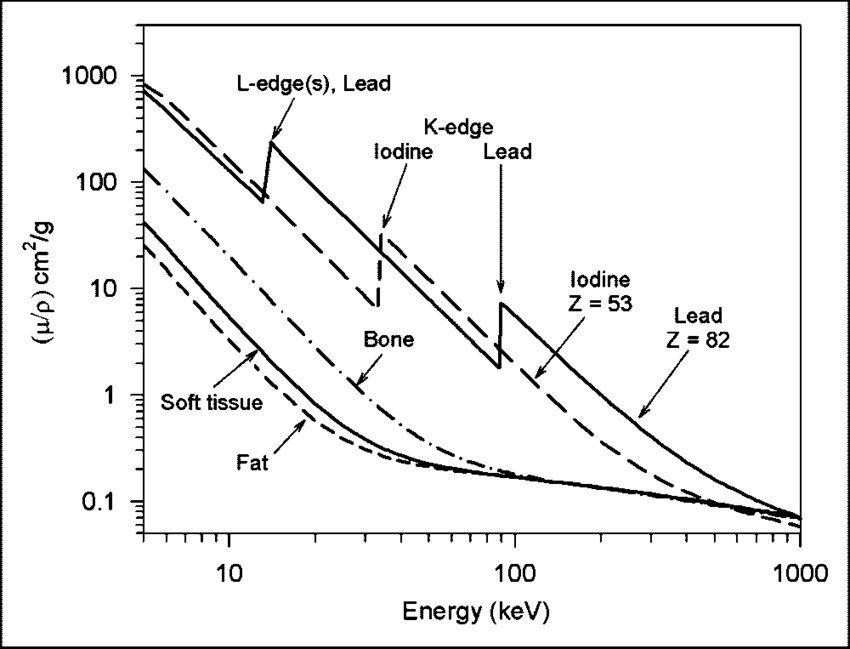
\includegraphics[width=0.7\textwidth]{figures/intro/attenuation-for-several-materials.png}
  \caption{The mass attenuation coefficient as a function of photon energy for several materials encountered in diagnostic X-ray imaging \cite{seibert2005x}} \label{fig:attenuation-for-several-materials}
\end{figure}

There are different methods to acquire the final image containing blood vessels only (angiogram). First, the more popular technique, Digital Subtraction Angiography (\gls{dsa}) is discussed.

\subsection{Digital Subtraction Angiography}
As digitization of images was introduced and manipulation of digitized information became widely used in the 1970s, Digital Subtraction Angiography (\gls{dsa}) became practical \cite{jeans1990development}. In this method, an image is taken before injecting the contrast agent into the blood vessel. Later, this pre-contrast image is being subtracted from the images acquired at different times during the movement of the contrast agent so that only structures filled with  the agent are visualized and irrelevant anatomic features disappear \cite{levin1984digital}. Such procedure can be seen on Figure \ref{fig:/angio-frames}.

\begin{figure}[htpb]
  \centering
  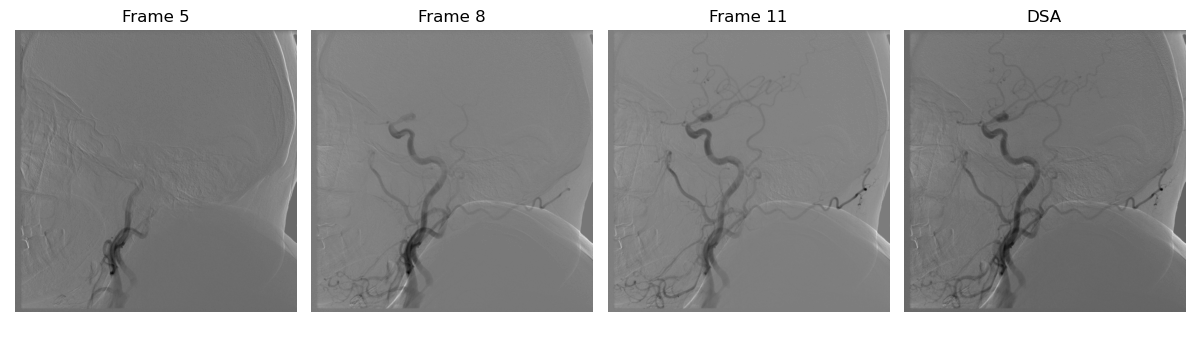
\includegraphics[width=1\textwidth]{figures/intro/angio-frames.png}
  \caption{Frames captured at different times and the \gls{dsa} image} \label{fig:/angio-frames}
\end{figure}

\gls{dsa} is a potent imaging technique that can give precise details about the structure and operation of the vascular system. It can be used to identify a variety of vascular conditions, including aneurysms \cite{chappell2003comparison}, peripheral artery disease \cite{fleischmann2006ct}  and coronary artery disease \cite{ambrose1988angiographic}.

Unfortunately, the procedure has some drawbacks. The injection of contrast material is one of the most common risks associated with \gls{dsa}. While the material is generally safe, allergic reactions or other adverse reactions are possible \cite{tramer2006pharmacological}. Another concern is the radiation exposure induced by X-rays, which should always be minimized in medical applications \cite{lange2006randomized}. Digital variance angiography is a viable solution to these issues.


\subsection{Digital Variance Angiography}

Digital variance angiography considers the variation that occurs during picture acquisition. Instead of capturing a single fully exposed image during the procedure, several underexposed images are taken.

\section{Image Processing}

An image can be thought of as a two-dimensional function, $f (x, y)$ where $x$ and $y$ are spatial coordinates. The intensity of the image is defined as the amplitude of $f$ at any given pair of coordinates $(x, y)$. We refer to the image as a digital image when $x$, $y$ and the intensity values of $f$ are all finite, discrete quantities. Processing digital images using a computer is referred to as the field of digital image processing \cite{gonzalez2018digital}.

\subsection{Intensity Transformations}

The following is the general formula for intensity transformations:

\begin{equation}
    g(x,y)=T[f(x,y)]
    \label{eq:intensity-transform}
\end{equation}

where $f(x,y)$ is the input image, $g(x,y)$ is the output image and $T$ is an operator on $f$ defined over a neighborhood of point $(x,y)$. When a neighborhood is of size 1x1, $g$ is determined solely by the value of $f$ at a single point $(x,y)$ and $T$ can be reduced to the form:

\begin{equation}
    s=T(r)
    \label{eq:intensity-transform-simplified}
\end{equation}

where $s$ and $r$ denote the intensity after and before the intensity transformation respectively.  The simplest intensity transformations are contrast stretching and thresholding which can be seen on Figure \ref{fig:/stretching-and-thresholding}. By utilizing these methods, one can achieve higher contrast than the original. Also, binary images can be created if $T$ is a thresholding function.

\begin{figure}[htpb]
  \centering
  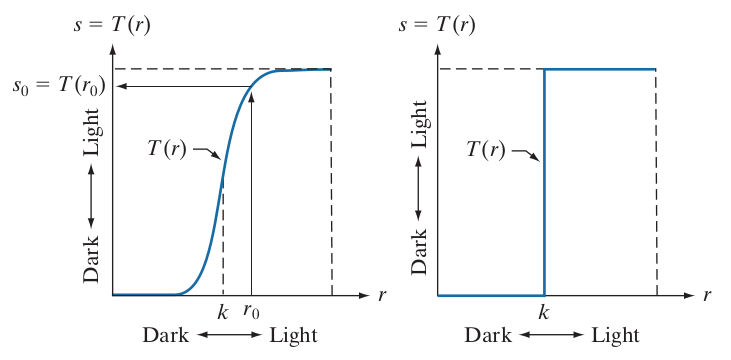
\includegraphics[width=0.7\textwidth]{figures/intro/stretching-and-thresholding.png}
  \caption{Intensity stretching and thresholding \cite{gonzalez2018digital}} \label{fig:/stretching-and-thresholding}
\end{figure}

If the majority of an image's details are concentrated in a dark, narrow region of the histogram, using power law transformation can significantly improve visibility. These transformations can be expressed as the following:

\begin{equation}
    s=r^{\gamma}
    \label{eq:power-law}
\end{equation}

where $\gamma$ is a positive constant which can be tuned for the desired needs as shown on Figure \ref{fig:/power-law}.

\begin{figure}[htpb]
  \centering
  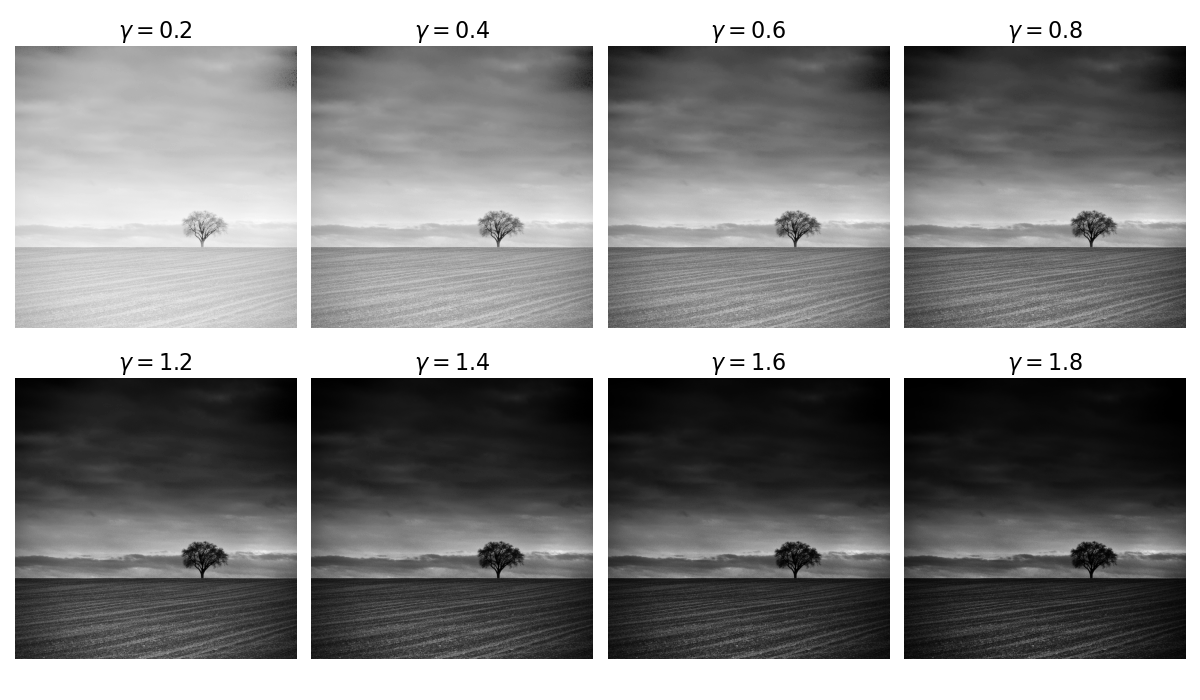
\includegraphics[width=1\textwidth]{figures/intro/power-law.png}
  \caption{Power law transformations with various $\gamma$ values \cite{tree-img}}
  \label{fig:/power-law}
\end{figure}


Another effective way to enhance the global contrast of images is applying histogram equalization. The basic idea is to distribute intensities more evenly when the image is represented by a narrow range of intensity values. Figure \ref{fig:/unequalized_hist} shows an image with its histogram.  The histogram is constrained to a narrow region which results poor contrast.

\begin{figure}[htpb]
  \centering
  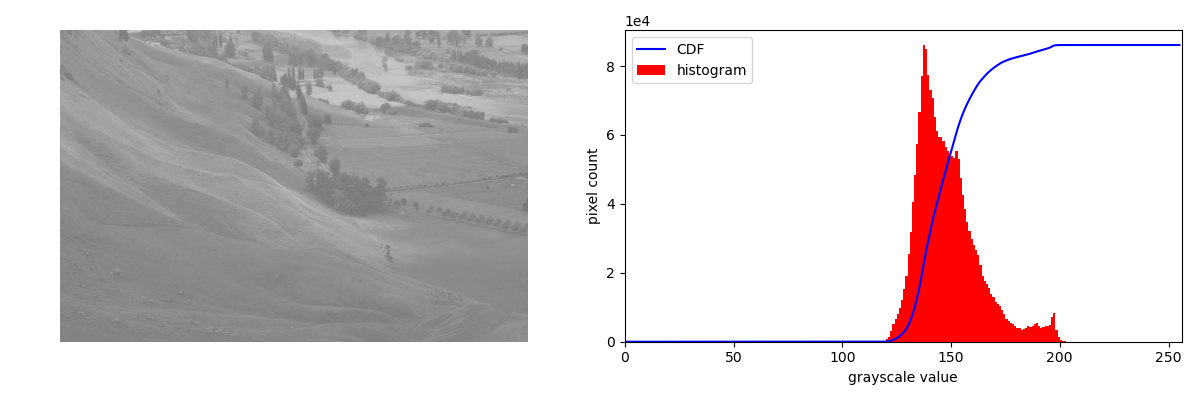
\includegraphics[width=1\textwidth]{figures/intro/unequalized_hist.png}
  \caption{Original image and its histogram \cite{capper2006unequalized} \cite{bradski2000opencv} }
  \label{fig:/unequalized_hist}
\end{figure}

Ideally, the cumulative distribution function  \gls{cdf} is linearized across the value range. During histogram equalization, the values from the original narrow range are being mapped to the full range. Here, only the output is shown, the step-by-step algorithm can be found in the references \cite{gonzalez2018digital}.

\begin{figure}[htpb]
  \centering
  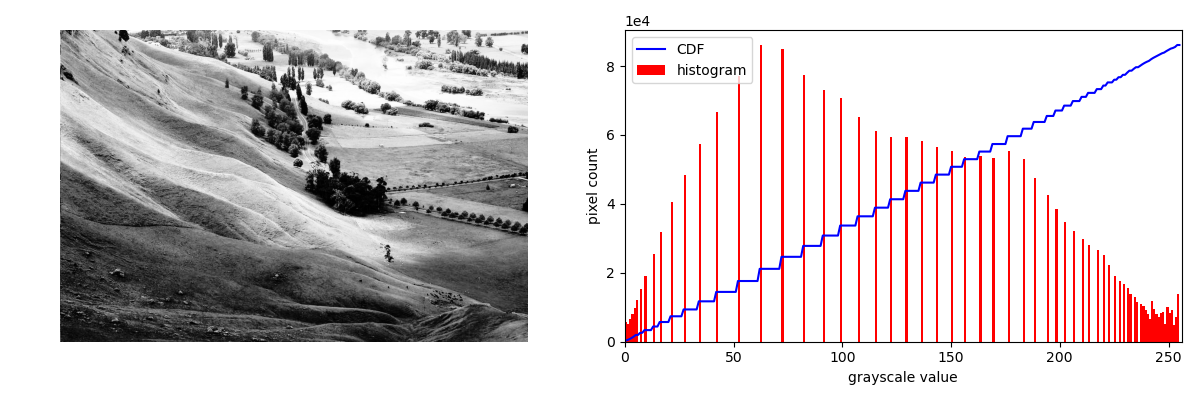
\includegraphics[width=1\textwidth]{figures/intro/equalized_hist.png}
  \caption{Equalized image and its histogram \cite{bradski2000opencv}}
  \label{fig:/equalized_hist}
\end{figure}

However, when the approach is applied globally, the final output might not be as desired. As it can be seen on Figure \ref{fig:/global-hist-eq}, the dark background's fine details are emphasized, but the characteristics of the face are lost in the foreground. One solution can be applying histogram equalization locally in order to preserve previously visible features while exposing predominantly hidden ones.

\begin{figure}[htpb]
  \centering
  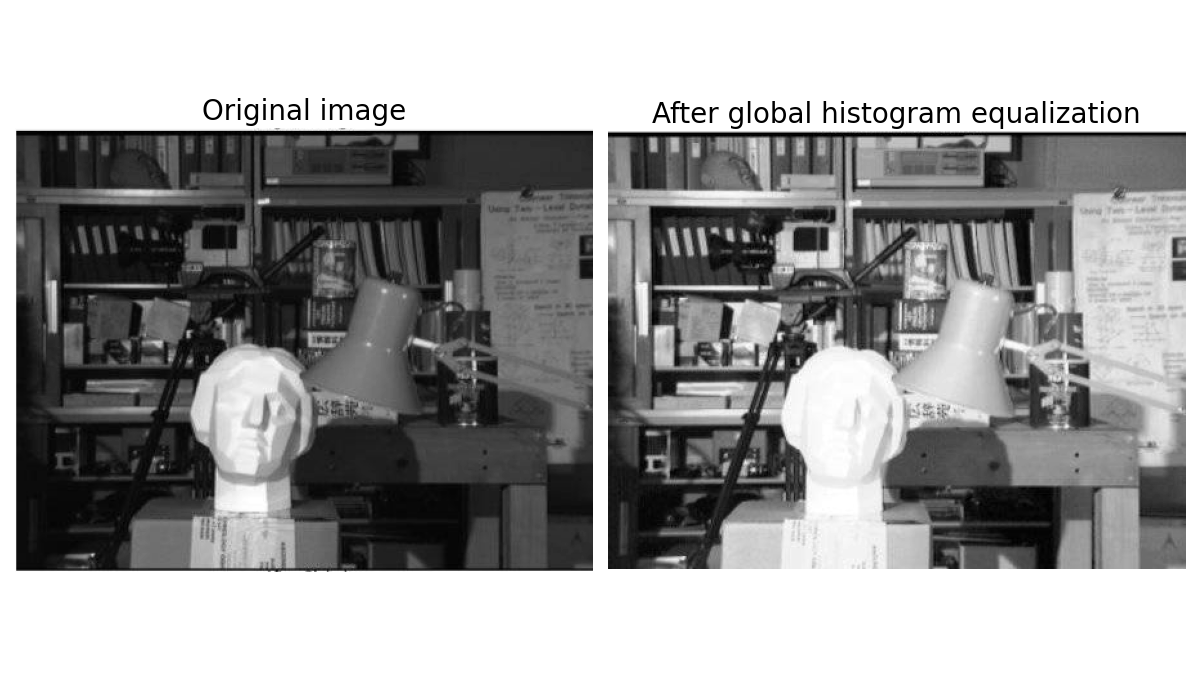
\includegraphics[width=0.8\textwidth]{figures/intro/global-hist-eq.png}
  \caption{Side effects of global histogram equalization \cite{bradski2000opencv}}
  \label{fig:/global-hist-eq}
\end{figure}

The suggested approach is called \gls{clahe} (Contrast Limited Adaptive Histogram Equalization) \cite{pizer1987adaptive}. Instead of equalizing the histogram globally, the image is partitioned into equal-sized regions known as tiles, each of which is subjected to individual histogram equalization as previously demonstrated. By simply doing so, noise might be amplified in near-constant regions. To prevent this, before applying histogram equalization, pixels that are above the given contrast limit in any histogram bin are clipped and evenly distributed to other bins. Finally, tile boundary artifacts are eliminated using bilinear interpolation. The outcome is shown in Figure \ref{fig:/intro-clahe}. While histogram equalization enhanced successfully the visibility of the dark background, there was also a slight improvement in the visibility of the face in the foreground.

\begin{figure}[htpb]
  \centering
  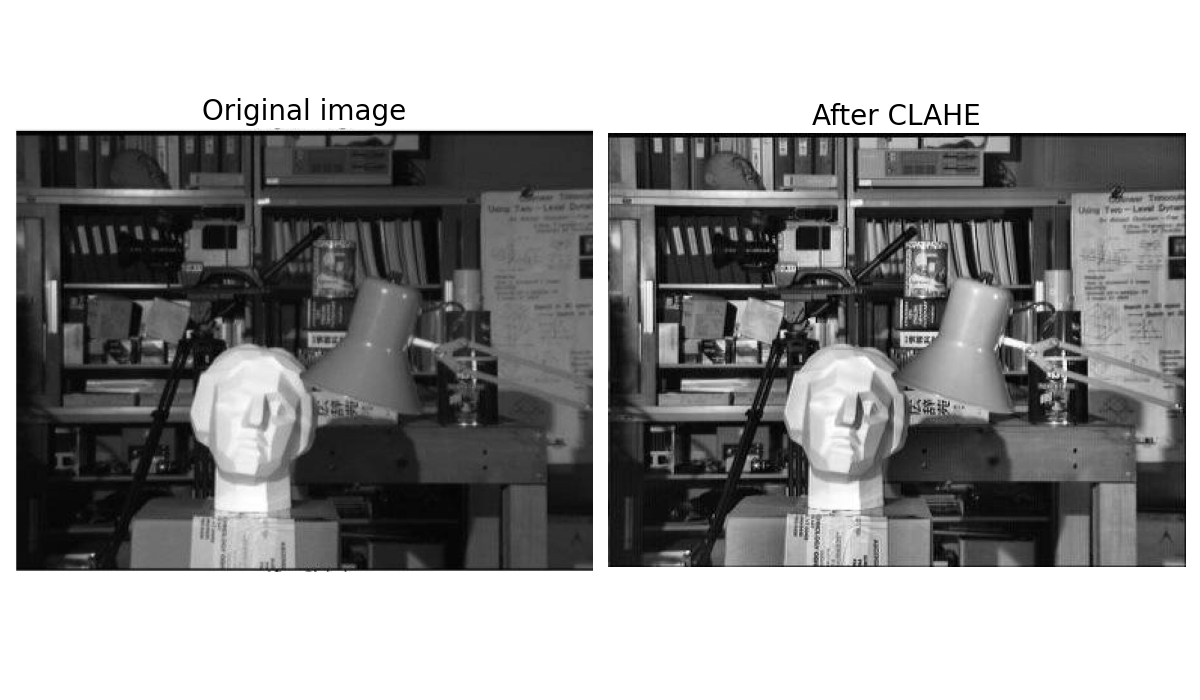
\includegraphics[width=0.8\textwidth]{figures/intro/clahe.png}
  \caption{\gls{clahe} with clipLimit=2.0 and tileGridSize=(8,8)  \cite{bradski2000opencv}}
  \label{fig:/intro-clahe}
\end{figure}

As it was covered in this subsection, intensity transformations provide a useful toolkit when contrast enhancement is required. However, if image smoothing or sharpening is desired, spatial filtering must be used.


\subsection{Filtering in Spatial Domain}

Spatial filtering modifies an image by replacing the value of each pixel by a function of the values of the pixel and its neighbors \cite{gonzalez2018digital}. The general formula for linear spatial filtering can be written in these forms:

\begin{equation}
	g(x,y)=\sum_{s=-a}^{a}\sum_{t=-b}^{b}w(s,t)f(x+s,y+t)
	\label{eq:correlation}
\end{equation}

\begin{equation}
	g(x,y)=\sum_{s=-a}^{a}\sum_{t=-b}^{b}w(s,t)f(x-s,y-t)
	\label{eq:convolution}
\end{equation}

where $g(x,y)$ is the output pixel, $w$ is the kernel, $f(x,y)$ is a pixel of the original image, $s$ is the index iterating in the vertical direction within distance $2a$ and $t$ is the index iterating in the horizontal direction within distance $2b$. Here, odd-sized, symmetric kernels are discussed, mostly 3x3. Figure \ref{fig:/convolution} illustrates the process.

\begin{figure}[htpb]
  \centering
  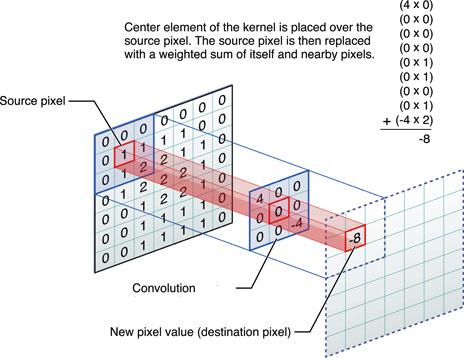
\includegraphics[width=0.8\textwidth]{figures/intro/convolution.png}
  \caption{The mechanics of linear spatial filtering using a 3 × 3 kernel \cite{basavarajaiah2019convolution}}
  \label{fig:/convolution}
\end{figure}

The method consists of moving the kernel's center over an image and computing the product sum at each position. Essentially, Equation \ref{eq:correlation} is a correlation between the kernel and the image. In Equation \ref{eq:convolution}, which is known as convolution, minus signs are used in the arguments of $f$. However, convolution and correlation provide the same result when the kernel is symmetric. In this thesis, convolution, Equation \ref{eq:convolution}, is preferred and used subsequently.

Many times, one wishes to blur or sharpen an image. First, it is covered how the prior can be obtained. The most convenient kernel for this purpose is a lowpass gaussian kernel:

\begin{equation}
	w(s,t)=e^{-\frac{s^{2}+t^{2}}{2\sigma^{2}}}
	\label{eq:lowpass-gaussian-spatial}
\end{equation}

where $\sigma$ is the standard deviation.  As the numerator of the exponent represents the distance from the center of the kernel, the expression can be simplified to the following form:

\begin{equation}
	w(r)=Ke^{-\frac{r^{2}}{2\sigma^{2}}}
	\label{eq:lowpass-gaussian-spatial-r}
\end{equation}

where $r$ is the distance from the center of the kernel. In image processing, filter kernels are used in their discrete forms because images contain finite number of non-zero-sized pixels. Therefore, a 3x3 lowpass gaussian kernel with $\sigma=1$ is used as it can be seen on Figure \ref{fig:/lowpass-gaussian-spatial-discrete}.

\begin{figure}[htpb]
  \centering
  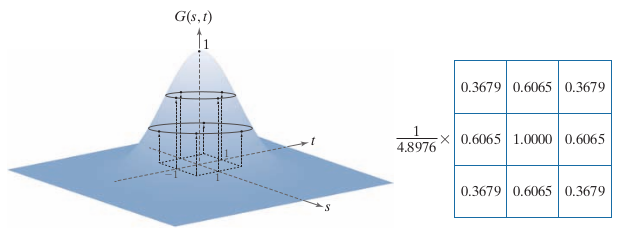
\includegraphics[width=0.8\textwidth]{figures/intro/lowpass-gaussian.png}
  \caption{Normalized 3x3 gaussian kernel \cite{gonzalez2018digital}}
  \label{fig:/lowpass-gaussian-spatial-discrete}
\end{figure}

Figure \ref{fig:/lowpass-gaussian-example} shows the effects of convolving an image with lowpass gaussian kernels. As it can be seen, bluring is noticeable on the branches of the tree even when the 3x3 kernel is used. The blurring becomes more obvious if the kernel size is extended to 7x7 because the kernel covers more nearby pixels.

\begin{figure}[htpb]
  \centering
  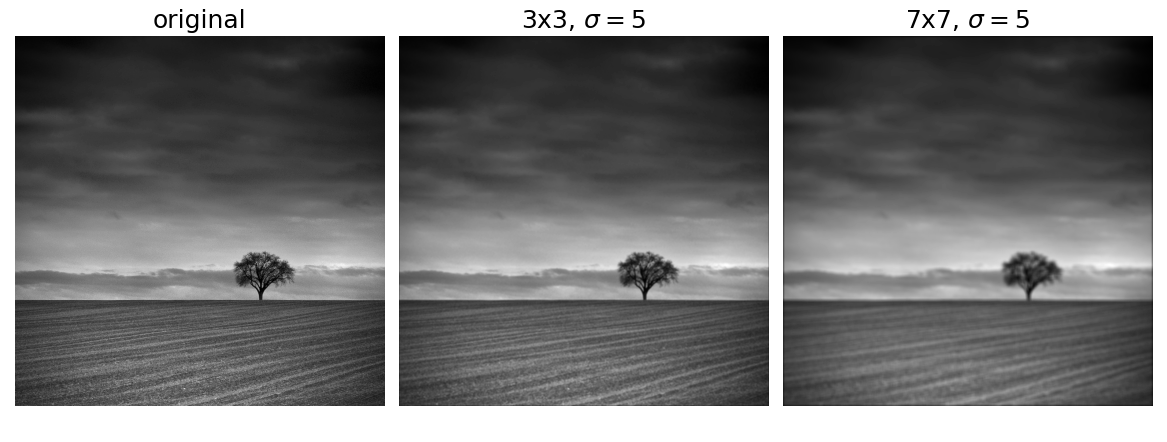
\includegraphics[width=1\textwidth]{figures/intro/lowpass-gaussian-example.png}
  \caption{Image convolved with lowpass gaussian kernels \cite{tree-img}}
  \label{fig:/lowpass-gaussian-example}
\end{figure}

As it was mentioned earlier, another common image manipulation technique is sharpening.


\subsection{Filtering in Fourier Domain}

hello from fourier domain